\chapter{Theory}
    \label{chap:theo}
    
    \section{FINken Modelling}
    \label{sec:theomodel}
    
    \subsection{Quadcopter modelling}
    \label{sec:copterModel}
    \tikzstyle{force} = [ultra thick, -latex]
    \tikzstyle{myTest3}=[x={(-0.510cm,0.410cm)},z={(0cm,-0.870cm)},y={(0.810cm,0.310cm)}]
    \tikzstyle{myTest}=[x={(-0.5cm,0.5cm)}, y={(0.5cm,0.5cm)}, z={(0cm,-1.0cm)}]
    \tikzstyle{myTest2}=[x={(-0.71cm,0.41cm)}, y={(0.71cm,0.41cm)}, z={(0cm,-0.82cm)}]
    \NewDocumentCommand{\DrawCoordinateAxis}{O{} m m m m m m}{%
        \def\XAxisMin{#2}
        \def\XAxisMax{#3}
        \def\YAxisMin{#4}
        \def\YAxisMax{#5}
        \def\ZAxisMin{#6}
        \def\ZAxisMax{#7}
        \begin{scope}[thin, gray, -latex]
            \draw [#1] (\XAxisMin,0,0) -- (\XAxisMax,0,0) node [left] {$x$};
            \draw [#1] (0,\YAxisMin,0) -- (0,\YAxisMax,0) node [right] {$y$};
            \draw [#1] (0,0,\ZAxisMin) -- (0,0,\ZAxisMax) node [right] {$z$};
        \end{scope}
    }%
    
    \begin{figure}[ht]
    \centering
    \begin{tikzpicture}[scale=1, auto, myTest3]
    
    \coordinate (o) at (0,0,0);
    
    % quadcopter arms
    \draw (5.25, -4.75, 0) -- (4.75, -5.25, 0) -- (-5.25, 4.75, 0) -- (-4.75, 5.25, 0) -- cycle;
    \draw (5.25, 4.75, 0) -- (4.75, 5.25, 0) -- (-5.25, -4.75, 0) -- (-4.75, -5.25, 0) -- cycle;
    %quadcopter body
    \draw[fill=gray!20] (1, -1, 0) -- (1, 1, 0) -- (-1, 1, 0) -- (-1, -1, 0) -- cycle;
    %quadcopter rotors as circles
    \draw[fill=gray!50] (5,5,-0.1) circle (1.5);
    \draw[fill=gray!50] (-5,5,-0.1) circle (1.5);
    \draw[fill=gray!50] (5,-5,-0.1) circle (1.5);
    \draw[fill=gray!50] (-5,-5,-0.1) circle (1.5);
    %forces acting on the quadcopter
    \draw[force] (5,-5,0) -- (5,-5,-1) node[midway, right] {$F_{1}$};
    \draw[force] (-5,-5,0) -- (-5,-5,-1) node[midway, left] {$F_{2}$};
    \draw[force] (-5,5,0) -- (-5,5,-1) node[midway, right] {$F_{3}$};
    \draw[force] (5,5,0) -- (5,5,-1) node[midway, right] {$F_{4}$};
    \draw[force, dashed] (o) -- (0,0,4) node[midway, left,xshift=0.1cm] {$F_{G}$};
    %torques applied by rotors
    \draw[force] (5,-5,-0.5) ++(0+180:1) arc (-180:90:1)node[right,xshift=0.1cm] {$\tau_{1}$};
    \draw[force] (-5,-4,-0.5) arc (90:360:1)node[left,xshift=0.1cm] {$\tau_{2}$};
    \draw[force] (-5,5,-0.5)++(-180+180:1) arc (0:270:1)node[right,xshift=0.1cm] {$\tau_{3}$};
    \draw[force] (5,4,-0.5) arc (-90:180:1)node[right,xshift=0.1cm] {$\tau_{4}$};
    % pitch roll and yaw in their respective planes
    \begin{scope}[canvas is zx plane at y=0]
    \draw[-latex,thick] (0,-3) arc (270:135:3) node[left] {pitch $\theta$};
    \draw[dotted] (o) circle(3);
    \end{scope}
    \begin{scope}[canvas is zy plane at x=0]
    \draw[-latex,thick] (0,-2.5) arc (270:135:2.5)node[above] {roll $\phi$};
    \draw[dotted] (o) circle(2.5);
    \end{scope}
    \draw[-latex,thick] (0,-4,0) arc (270:70:4)node[right] {yaw $\psi$};
    \draw[dotted] (o) circle(4);
    %reference coordinate system
    \begin{scope}[shift={(0,-6,5)}]
    \DrawCoordinateAxis[thick, black]{0}{1}{0}{1}{0}{1}
    \end{scope}
    \end{tikzpicture}
    \caption{Forces and torques of a quadcopter}
    \label{fig:finkenDyn}
    \end{figure}
    
    
    For the simulation, at first, the basic physics behind a quadcopter have to be identified. 
    As V-REP provides a physics engine, in our case bullet \cite{bullet}, we will not build a complete physical model of the quadcopter in flight, but keep to what is necessary to simulate it in VREP.
    A quadcopter is an aircraft with 4 rotors. 
    In our simple case, the rotors are identical, mounted fix to the quadcopter body in the same $xy$-plane and have parallel thrust vectors pointing in the same direction. 
    At start of the simulation, the inertial coordinate system and the copters body coordinate system has identical $x,y,z$-axis. 
    However, when the copter moves, it's body coordinate system moves as well, keeping the copters center of mass at its origin, then denoted with $x_b, y_b, z_b$.
    
    When the rotor $i$ are powered, it turns with the angular velocity $\omega_i$, creating a force in the direction of the rotor axis, which is equivalent to the quadcopter body axis $z$, and a torque $\tau_i$ around the rotor axis.
    \begin{equation}
    F_i = k\omega_i^2, \tau_i = d\omega_i^2 + I_M\dot\omega_i
    \label{equ:forceAndTorque}
    \end{equation}
    
    The constant $k$ depends on air density and rotor geometry. $d$ is the drag constant for the rotor drive train and $I_M$ ist the moment of inertia of the rotor which adds a torque during angular acceleration. However, with the small diameters and lightweight plastic rotors, this contribution to the overall torque is comparatively small and can be omitted.
    
    For the whole copter, we get the combined force $F_{sum}$ with $F_{sum} = \sum_{i=1}^{4}{F_i}$ and the resulting thrust $F_b$ relative to the body with $F_b = (0, 0, F_{sum})^T$. For the torque in body frame angles, the rotation direction of the rotor have to be taken into account.
    \begin{equation}
    \tau_b =\begin{bmatrix}\tau_\phi \\ \tau_\theta \\ \tau_\psi \end{bmatrix} = \begin{bmatrix}cos(45)lk_{torque}(F_1 + F_2 - F_3 - F_4) \\ cos(45)lk_{torque}(-F_1 + F_2 + F_3  - F_4  ) \\ \sum_{i=1}^{4}{\tau_i} \end{bmatrix}
    \label{equ:torques}
    \end{equation}
    The rotor are mounted in distance $l$ from the copters center of mass and the copter arms form a $\ang{45}$ angle to the $x_b$- and $y_b$-axis, resulting in a distance of $cos(45)l$ to the axis which their thrust creates a force around\cite{luukkonen2011modelling}.
    
    To keep the copter in air, the forces generated by the thrust of the 4 rotors have to compensate the force $F_{G}$ generated by the weight of the quadcopter.
    
    \begin{equation}
    F_G = F_1 + F_2 +F_3 + F_4
    \end{equation}
    
    Now, that the forces and torques on the coper are modelled, the model can be integrated into V-REP, as the physics engine will compute the according movements.
    
    
    \subsection{Rotor Modelling}
    \label{sec:rotorTheory}
    
    Due to manufacturing tolerances and external influences as air stream, the forces $F_i$ and torques $\tau_i$ generated at a certain angular velocity $\omega$ as decribed in \ref{equ:forceAndTorque} is different for each rotor. 
    In the previous section \ref{sec:copterModel}, we assumed, that all the rotors are identical. 
    As this assumption doesn't hold, therefore a particle simulation was used to simulate the forces $F_i$ and torques $\tau_i$ of the rotors. 
    Using four particle objects with identical parameters, the model of section \ref{equ:forceAndTorque} can be used, but the particle simulation adds some noise which makes the copter behaviour more realistic. 
    The particle simulation was already included in V-REP's example quadcopter model and was only slightly modified.
    
    The particle simulation is used to simulate the airstream generated by the rotor. 
    The particle object can be configured with  particle size $s_{px}$, particle density $\rho_{px}$ and maximum number of particles $n_{px}$ it can hold. 
    A simulation of rotors spinning in a particle cloud would take to much computation time, so the  particles are generated below the rotor modeling the air stream. 
    In the following the physics behind this simulation are shown, assuming that the copter is hovering, that the free stream velocity $v_0$ of the air around the quadcopter is zero and that the air is incompressible, which is valid as long as stream velocity are well below the speed of sound \cite{Lautrup2011PhysicsContinuous}.
     Also, a homogeneous stream velocity under the whole rotor area is assumed which is sufficient accurate for this case. 
    
    Based on our assumptions, Momentum Theory gives us the thrust $F_i$ of a single rotor as a product  of the mass flow rate $\dot m$ and final speed $v_{final}$ of the air accelerated by the rotor  
    
    \begin{equation}
    F_i = \dot m v_{final} 
    \label{equ:momentum}
    \end{equation}
    
    This means, to simulate the thrust $F_i$ with the particle object, the mass of particles and the final stream velocity is needed.
    
    Neither the mass of the airstream nor the final stream velocity is easy to measure, but the thrust $F_i$ when hovering is easily calculated from the weight of the copter.
    \begin{equation}
    F_i = \frac{F_G} {4}, F_G = m_{copter} * g
    \end{equation}
    
    
    The mass flow rate $\dot m$, though not directly measurable,  can be obtained from the air density $\rho_{air}$, and the volumetric flow rate $\dot V$ through the rotor as shown in ¸\ref{equ:mfr}. 
    The air density is constant (we assume standard conditions), and the volumetric flow rate  depends on the area $A$ covered by the rotor and the air velocity in the rotor plane $v_{rotor}$.
    \begin{equation}
    \dot m = \rho_{air} \dot V = \rho_{air} A v_{rotor}
    \label{equ:mfr}
    \end{equation}
    
    Note, that the air stream velocity $v_{rotor}$ in the rotor plane is different from the final air stream velocity $v_{final}$ the air reaches behind the rotor. 
    This can be shown, as by the conservation of energy, the power $P$ the rotor puts into the air stream has to equal the energy $E_{kin}$ the air stream carries per time as in \ref{equ:consE} and \ref{equ:momentumEnergy}. 
    For the first derivative of the kinetic energy $E_{kin}$ in \ref{equ:Ekin} note that the velocity is considered constant during hovering.
    
    \begin{equation}
    P = F_i v_{rotor}
    \end{equation}
    \begin{equation}
    E_{kin} = \frac{1}{2} m v_{final}^2, \dot E_{kin} = \dot m \frac{v_{final}^2}{2}
    \label{equ:Ekin}
    \end{equation}
    
    \begin{equation}
    P = \dot E_{kin}
    \label{equ:consE}
    \end{equation}
    
    \begin{equation}
    F_i v_{rotor} = \dot m \frac{v_{final}^2}{2}
    \label{equ:momentumEnergy}
    \end{equation}
    
    Inserting \ref{equ:momentum} into \ref{equ:momentumEnergy} shows the relation between $v_{rotor}$ and $v_{final}$.
    \begin{equation}
    \dot m v_{final}  v_{rotor} = \dot m \frac{v_{final}^2}{2}
    \end{equation}
    \begin{equation}
     v_{rotor} = \frac{v_{final}}{2}
     \label{equ:airvelocities}
    \end{equation}
    
    With the air velocity $v_{rotor}$ in the rotor plane, the thrust $F_i$ of a rotor can be calculated from the rotor area $A$ and air densitiy $\rho_{air}$ which are known.
    \begin{equation}
    F_i = 2 \rho_{air} A v_{rotor}^2
    \label{equ:thrustAirflow}
    \end{equation}
    
    \ref{equ:thrustAirflow} and \ref{equ:airvelocities} together give a formula to determine the  velocity $v_{rotor}$  when the copter hovers.
    \begin{equation}
    v_{rotor}= \sqrt{\frac{ F_i}{2 \rho_{air} A}}
    \end{equation}
    
    As written in the introduction, the particle simulation includes the parameters particle density $\rho_{px}$, particle size $s_{px}$ and rate $\dot n_{px}$, meaning how many particles are created per time. 
    Particle density and particle size should be constant, as the air stream is considered incompressible, so when leaving poise, the particle rate has to change according to \ref{equ:mfr} \cite{deeg2006modeling}.
    
    The particles are spherical, with the particle size $s_{px}$ as the sphere's diameter, so the mass $m_{px}$ of a single particle can be calculated as in \ref{equ:Vandm}.
    \begin{equation}
    m_{px} = V_{px}  \rho_{px}  =  \frac{\pi}{6}s_{px}^3  \rho_{px},  V_{px}  = \frac{\pi}{6}s_{px}^3
    \label{equ:Vandm}
    \end{equation}
    
    The mass flow rate $\dot m$ of the particle is the product of particle rate $\dot n_{px}$ and the particle mass $m_{px}$.
    \begin{equation}
    \dot m =  \dot n_{px} m_{px}= \dot n_{px}  \frac{\pi}{6}s_{px}^3  \rho_{px}
    \label{equ_simmfr}
    \end{equation}
    
    During flight, if the air stream velocity $v_{final}$ changes, the mass flow changes as well according to \ref{equ:mfr}, so the mass flow rate needs to be expressed as a function of air stream velocity. 
    
    Equating \ref{equ_simmfr} with  \ref{equ:mfr} in \ref{equ:simmfrrealmfr} relates particle rate $n_{px}$ to the already known parameters particle mass $m_{px}$, air density $\rho_{air}$, rotor area $A$ and the final air stream velocity $v_{final}$ in \ref{equ:pxrate}.
    
    \begin{equation}
    \dot n_{px} m_{px} =  \rho_{air} A v_{rotor}
    \label{equ:simmfrrealmfr}
    \end{equation}
    
    \begin{equation}
    \dot n_{px} = \frac{\rho_{air} A}{m_{px}} v_{rotor} = \frac{\rho_{air} A}{2m_{px}} v_{final}
    \label{equ:pxrate}
    \end{equation}
    
    Now, the particle simulation can be parametrized based on the copter hovering. 
    But, all parameters except for air stream speed are constant.
    Thererefore,  the copter's dynamics can be simulated by connecting the air stream velocity to the throttle, so the copter's thrust will be adjusted accordingly.
    
    The thrust of the rotor can be expressed as \ref{equ:simThrust} by inserting \ref{equ:simmfr} into \ref{equ:momentumTheory}
    \begin{equation}
    F_i = \dot n_{px}  \frac{\pi}{6}s_{px}^3  \rho_{px} v_{final}
    \end{equation}
    
    Particle size $s_{px}$, mass $m_{px}$ and rate $\dot n_{px}$ can be arbitrarily chosen, as long as \ref{equ:simmfrrealmfr} is satisfied. See \ref{sec:implparticle} for the calculated values.
    
    

    

    
    \section{Vrep}
    \label{sec:theoryVrep}
    V-REP is a versatile, highly customisable simulation environment, mainly developed for robots. 
    It provides a rich set of functionalities which we use only a part off.  
    We make use of it's integration of the bullet physics engine, including a particle simulation, it's external Java API, the communication structure via signals, the possibility of Lua scripting inside the simulation, it's provided sensor-simulation and the scene visualisation.
    \begin{figure}[h!]
     \begin{center}
      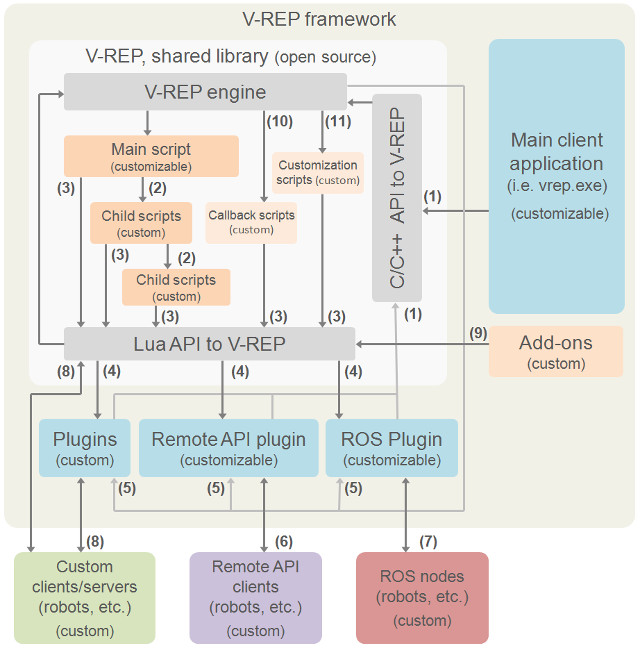
\includegraphics[scale=0.45]{vrepStruct.jpg}
     \end{center}
      \caption{Structure of the VREP-framework from \url{http://www.coppeliarobotics.com/helpFiles/en/images/writingCode1.jpg} 13.10.2015 \label{fig:vrepStruct}}
    \end{figure}
    
    The V-REP main client application provides the basis vor the simulation. 
    V-REP bases on scenes in which the simulation settings and scenes are saved. 
    To run a simulation, the necessary objects need to be added to the scene. 
    An object can be a dummy object with no physical properties, a 3-D shape either imported via an .stl-file or created directly in V-REP. 
    V-REP already provides a library of objects, starting with sensors and continuing with whole robots. 
    An example are force sensors which can be used to connect object. 
    Then, the force sensor transmits the resulting forces and torques during the simulation and can be set to break when exceeding a certain threshold. 
    Connecting objects without force sensors can be used to separate physical simulation and visual representation. 
    The connection becomes static, so a complex, but visually appealing mesh shape can be attached to a simpler shape with appropriate physical parameters. 
    Thereby, physical simulation calculation are performantly done on the simple, and as V-REP provides several visibility layers, the user sees only the complex shape.
    
    V-REP provides several possibilities to extend the simulation programmatically. 
    The easiest and best integrated way are Lua-scripts. Lua scripts can be attached to simulation objects and are handles within the simulation environment. 
    When choosing non-threaded child scripts, they get executed every simulation step and can influence scene objects via a comprehensive API. 
    A V-REP simulation step consists of several sections. 
    To execute parts of the script only at certain points, the current simulation status can be checked before executing code.  
    The downside of these Lua-scripts is, that they are stored inside the binary scene file. 
    Thus, it's difficult to put them under version control or do collaborative work. 
    As the Lua-Engine inside V-REP provides full Lua support, this can be avoided by using the internal scripts only to import and call the actual scripts that are stored outside the scene. 
    In section \ref{sec:implSoftware} is described how we handled this problem in detail.
    
    If Lua doesn't offer the needed performance or functionalities, the second way to build deeply integrated software is the internal C++ API for plugins.
    The most flexible, but least performant way is the remote API of V-REP.
    Providing an API for Java, Matlab, Python and Urbi, it interacts with many programming languages.
    However, the functionality provided by the remote API is limited compared to the internal API for Lua or C++.
    For the remote API, V-REP needs to start a server that the client connects to.
    This is also possible over network, so the computation load can be distributed between different machines.
    
    For communication inside V-REP, global custom variables can be used. As the access to those is not supported by the remote API, a more flexible way are \emph{Signals}. \emph{Signals} can be of String, Integer or Float type and are globally accessible  in the current scene. 
    
    


    
    
    \section{Communication V-REP-Quadrocopters}
    \label{sec:comm}
    \textbf{\textit{Goal}:} our mixed reality simulation needs a dependable link of communication between the V-REP simulation environment and the flying quadrocopters. 
    The Quadcopter needs to stream its telemetry data in real-time to the V-REP, and the reverse communication is needed as well.\\
    The simulated quadrocopters that we have in the V-REP are divided into two categories: real and virtual representations.\\ 
    The real are replicating the physical flying quadrocopters. They should perform the same flying manoeuvres as those flying in the real environment. 
    In order to make the model replicate this behaviour, the flying quadrocopter must send its linear and angular velocity, its pitch yaw and row and other parameters in real time to its representation model in V-REP. 
    The simulation model should also send the readings from its proximity sensors to the flying quadcopter thus providing it with information from a virtual sensor. \\
    The virtual quadrocopters are purely simulation quadcopter objects, that exist only in the V-REP simulation environment. Their purpose is to interact with the real quadrocopters for example to avoid collisions and thus making the first steps in the swarm research. The virtual quadrocopters have to be seen in the Paparazzi ground station as if they are real physical quadrocopters. It means that all the ground station agents like message logger, the signal plotting, attitude indicator, artificial horizon and other displays have to be updated with adequate information coming from the virtual quadrocopters in the V-REP.
    
    The communication between the V-REP quadrocopter models and the physical quadrocopters passes through several software components, which are depicted on figure \ref{fig:communication} and discussed in the next chapters.
    
    \begin{figure}[h!]
     \begin{center}
      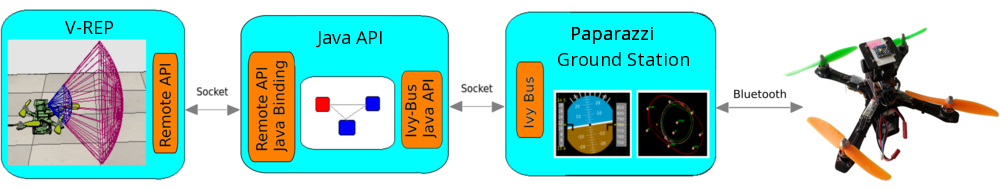
\includegraphics[scale=0.15]{communication.png}
     \end{center}
      \caption{communication V-REP - Quadrocopter\label{fig:communication}}
    \end{figure}
    
\subsection{V-REP Remote API}
    V-REP provides several means of communication with an external application. One of them is the Remote API, which allows to control a simulation (or the simulator itself) from an external application or a remote hardware (e.g. real robot, remote computer, etc.). The V-REP remote API is composed by approximately one hundred functions that can be called from a C/C++ application, a Python script, a Java application, a Matlab/Octave program, an Urbi script, or a Lua script. The remote API functions are interacting with V-REP via socket communication in a way that reduces lag and network load to a great extent.
    
\subsection{Java API}
    Java API is the external program, that we have implemented to communicate with V-REP through the Remote API.
    We have chosen to implement our external program, communicating with the V-REP, in the Java programming language regarding the following advantages: Java's platform independence allows to run the external program even on different machine with different operating system than the one used for running the V-REP environment.  Java is object-orientated which favours the use of design patterns and highly abstraction layers, which allows us to write an API that is modular, reusable and can later be easily extended to support other mixed-reality scenarious. Java also associates documentation with the actual code. The JavaDoc produces browsable documentation from the comments written in the code, which will be useful for anybody who wants to extend the project\\
    The implementation and architecture of the Java API is duscussed in details in \ref{sec:implementation}. The purpose of the Java application is to serve as a communicating bridge between the Paparazzi Ground Station and the V-REP. It detects all quadrocopters in the V-REP simulation, builds their virtual representations and feeds the models with real-time data.
    
\subsection{Ivy Bus}

Ivy Bus is a simple protocol and a set of open-source (LGPL) libraries and programs that allows applications to broadcast information through text messages, with a subscription mechanism based on regular expressions. Ivy libraries are available in C, C++, Java, Python and Perl, on Windows and Unix boxes and on Macs. \\
The Paparazzi Ground Station uses the Ivy Bus as a means of communication between the different software components. Figure \ref{fig:paparazziGS} depicts the communication structure in the Paparazzi Ground Station, in which the different agents communicate with each other by sending messages on the Ivy-Bus.

\begin{figure}[h!]
 \begin{center}
  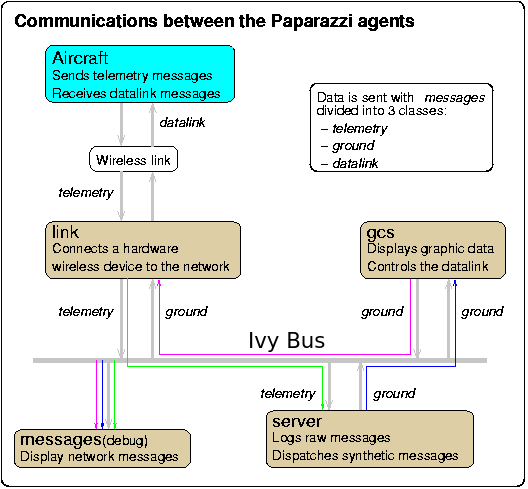
\includegraphics[scale=0.7]{paparazzi_gs.png}
 \end{center}
  \caption{Ivy-Bus in Paparazzi Ground Station\label{fig:paparazziGS}}
\end{figure}

The UAV (in blue) is streaming its telemetry data to the ground control station, which is received by the link. The \textbf{link} agent manages the ground-based radio modem and distributes the received messages to the other agents across the Ivy-Bus.

The Ivy Bus is an example of a publisher-subscriber protocol, in which senders of messages, called publishers, does not  explicitly specify the address of the receiver, but just send the message on one, shared by all nodes, bus. The recipients, called subscribers, which are interested in the message will accept it and the others will ignore it. The publisher-subscriber is a many to many communication model in which publishers are loosely coupled to subscribers - there is no space, flow and time coupling. This means that the publishers does not have to know the addresses of the subscribers and even does not need to know of their existence. Each can operate normally without the other and can continue its thread of execution regardless if the subscriber has received the message or not. It also provides scalability, which means that we can “attach” our Java API to the Ivy-Bus and start publishing and listening for messages without changing any line of source code in the Paparazzi Ground Station software.

In the publisher-subscriber model, subscribers typically receive only a subset of the total messages published. The process of selecting messages for reception and processing is called filtering. There are two common forms of filtering: topic-based and content-based.
In a topic-based system, messages are published to "topics" or named logical channels. Subscribers in a topic-based system will receive all messages published to the topics to which they subscribe, and all subscribers to a topic will receive the same messages. The publisher is responsible for defining the classes of messages to which subscribers can subscribe.
In a content-based system, messages are only delivered to a subscriber if the attributes or content of those messages match constraints defined by the subscriber. The subscriber is responsible for classifying the messages. Both filtering techniques are depicted in figures \ref{fig:pubsubsc_topic_based} and \ref{fig:pubsubsc_content_based}.

The Ivy Bus is a content-based publisher-subscriber and uses regular expressions for the message filtering.

\begin{figure}[!tbp]
  \centering
  \begin{minipage}[b]{0.4\textwidth}
    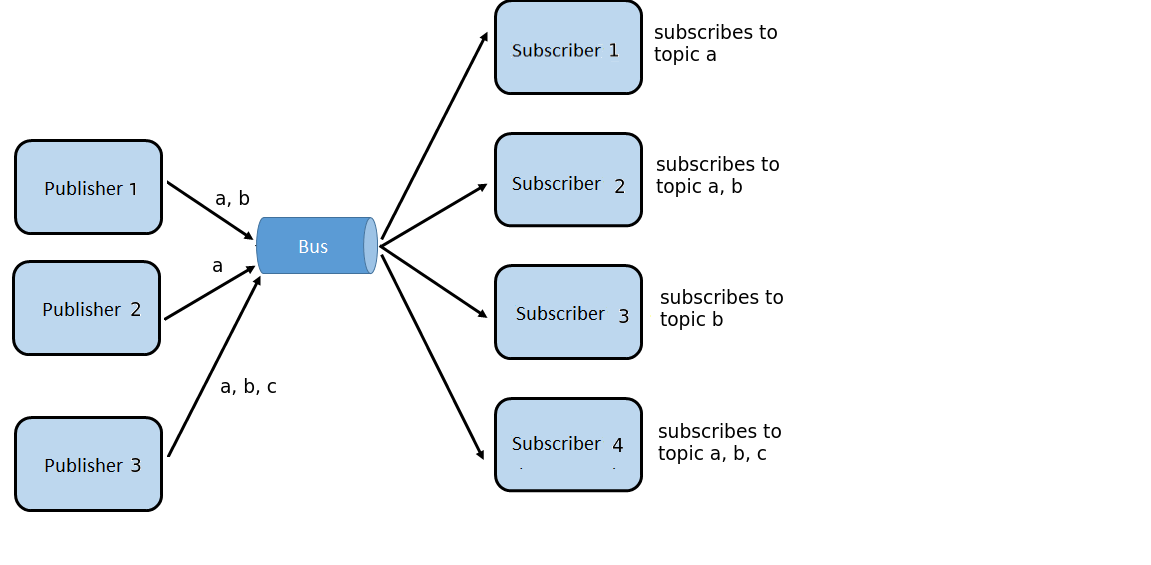
\includegraphics[scale=0.4]{pubsubsc_topic_based.png}
    \caption{Topic-based publisher-subscriber \label{fig:pubsubsc_content_based}}
  \end{minipage}
  \hfill
  \begin{minipage}[b]{0.4\textwidth}
    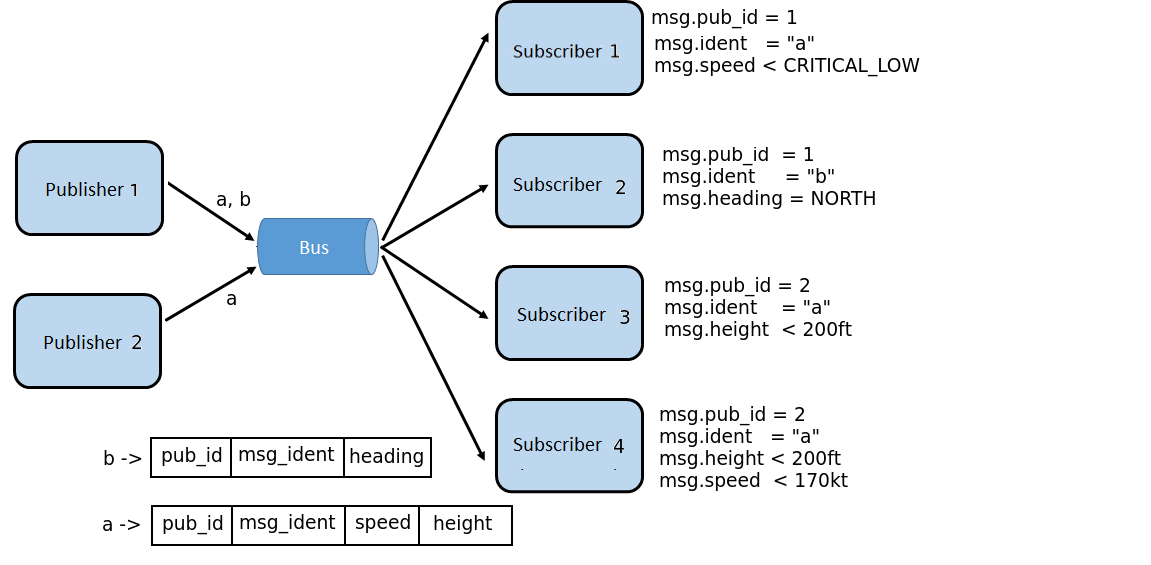
\includegraphics[scale=0.4]{pubsubsc_content_based.png}
    \caption{Content-based publisher-subscriber \label{fig:pubsubsc_topic_based}}
  \end{minipage}
\end{figure}

\subsection{Communication}
\label{sec:communication}

The communication between V-REP and the quadrocopters passes through the Java API, which serves as a bridge between them. In fact the Java API does not communicate directly with the quadrocopter, but connects to the Ivy-Bus in the Paparazzi GS and can thus subscribe to the messages caring the telemetry data and also publish messages which will eventually be send to the quadrocopter by the link agent. On the other hand it uses the V-REP Remote-API to exchange information and provide the V-REP quadrocopter models with the data retrieved from the Ivy-Bus messages.\\ 
Since we wanted to create a modular and reusable API, that can be used for other mixed-reality scenarios, the Java API was created with the idea in mind to be distributed, modular and rely on many abstraction layers.\\ 
The API development has followed the requirement-driven principles and its main tasks are described in the following paragraphs. The implementation of the described bellow requirements in described in \ref{sec:commImplementation} of \ref{sec:implementation}.

\subsubsection{V-REP-Remote API specific requirements}
\label{sec:requirementsVREP}

Below is a description of the requirements for the Java API which is responsible for the connection and communication with the V-REP environment. Its implementation is described in \ref{sec:vrepImplementation} of \ref{sec:implementation}.

\paragraph{Connection to V-REP through the Remote API}

There should be implemented a mechanism that enables to establish connection to the V-REP simulation. The connection should be able to be disconnected and reconnected at any time. Since the Remote API is based on a socket connection, it should be possible to connect to a V-REP server, situated on another machine, by specifying its IP address and port number. This will allow to run the V-REP simulation on a remote, powerful computer and thus release the local computer from having to deal with the simulation and communication program at the same time.

\paragraph{V-REP scene object and scene representation}\label{sceneobject}
The V-REP scene objects have to be represented as individual classes in order to be able to easily distinguish them and work with their properties. The class representing the scene object must have as fields the properties describing the simulation object - linear and angular velocity, position and orientation. The V-REP scene object hierarchy should also be implemented by using inheritance and composition object oriented techniques. \\
The Java API should provide methods to retrieve all scene objects from the V-REP scene and store them in a virtual scene representation for later use.\\
Since our quadrocopters are represented as shape objects and typically a V-REP scene contains at least 20 shape objects by default, there should be implemented a scanner that retrieves the quadrocopters from the scene. The scanner must be able to retrieve the virtual and real quadrocopters in a separate containers.

\paragraph{Continuous data exchange between quadrocopter instances and V-REP}

As mentioned at the beginning of \ref{sec:comm} we divide our quadrocopters in virtual and real representation. The virtual representations exist only in the V-REP scene, but they have to be visible in the paparazzi ground station as if they are real flying drones. It means that all the quadrocopter flying parameters have to be sent to the paparazzi ground station as messages. It becomes clear that the virtual quadrocopters have to be provided continuously with live data from the V-REP - linear/angular velocity, position and orientation. The real quadrocopter representations does not need to be provided with V-REP parameters, since its velocity, orientation and height are coming from the physical flying drone, but it has to be provided with data from its proximity sensor scene objects. The update with V-REP data should have a frequency equal to the simulation step used - 50 ms by default.\\
The real quadrocopter representation get provided with velocity, orientation and height from the physical flying quadrocopter and this data have to be provided to the V-REP quadrocopter object in order to fly like the physical one. This is the inverse communication from quadrocopter to V-REP and is realized with V-REP signaling mechanism. The update is done each time a new message has been received by the physical drone and its frequency depends on how often the messages are streamed from the copter and the communication latency. In order to achieve a realistic flying manuevers and have minimum drift the update should not exceed 20 ms.

\subsubsection{Ivy Bus specific requirements}
\label{sec:requirementsIVYBus}
\paragraph{Ivy Bus connection}
Each participant which wants to exchange information on the Ivy-Bus is described as a singular and independent bus node. In our program the participants that want to exchange data on the Ivy-Bus are the virtual and real representations of the quadrocopters. There should be designed a class, which allows the connecting on the bus, publishing and subscribing to messages. The quadrocopter representations have to inherit from it or composite it and thus become independent bus nodes.

\paragraph{Message retrieval and subscription}
\label{par:messageRetrieval}

All the messages that the paparazzi software uses are described in a xml file called \textit{messages.xml}, residing in the \textit{/paparazzi/conf/} directory. The following listing is an example of the messages file containing two messages.

\begin{lstlisting}[basicstyle=\tiny, caption={Message Xml definition}, label={lst:MessageXml}, language = Xml]
<msg_class name="telemetry">
 <message name="AIRSPEED" id="54">
    <field name="airspeed" type="float" unit="m/s"/>
    <field name="airspeed_sp" type="float" unit="m/s"/>
    <field name="airspeed_cnt" type="float" unit="m/s"/>
    <field name="groundspeed_sp" type="float" unit="m/s"/>
  </message>
  
  <message name="SONAR_ARRAY" id="216">
	<field name="sonar_front" type="uint16" alt_unit="cm"/>
	<field name="sonar_right" type="uint16" alt_unit="cm"/>
	<field name="sonar_back" type="uint16" alt_unit="cm"/>
	<field name="sonar_left" type="uint16" alt_unit="cm"/>
  </message>
	
	  . . . . 
	  
</msg_class>
\end{lstlisting}

In order to make the subscription and publishing of messages on the bus easier, each message should be represented as a corresponding class containing the message fields with its type and units.

There should be implemented a class, which reads the \textit{messages.xml} file and creates an instance of the message class for each message. \\
Once the messages are retrieved, the Ivy-Bus node should be capable of subscribing and publishing of any of the retrieved messages. The subscription should by dynamic and allow to subscribe to a new messages even at runtime. \\
Once a message has been received, the Ivy-Bus node should provide the instance of the received message and its fields should contain the actual sensor values.\\
Since our mixed reality scenario can involve many flying quadrocopters, there will be published the same messages but from different copters. In this case the messages are identified with the drone id number.
Another requirement is that the Ivy-Bus node have to subscribe just to the messages published from the copter that it was assigned to and not receive the same messages from the other copters.

\subsubsection{Application specific requirements}
\label{sec:requirementsApplication}

\paragraph{Aircraft retrieval}
\label{par:aircraftRetrieval}
The paparazzi software stores important information about the quadrocopters in an Xml file stored in \textit{/paparazzi/conf/conf.xml}

\begin{lstlisting}[basicstyle=\tiny, label={lst:AircraftXml}, language = Xml]
  <conf>
    <aircraft
      name="Quad_Lia_ovgu_01"
      ac_id="1"
      airframe="airframes/ovgu/free_flight.xml"
      radio="radios/spektrum.xml"
      telemetry="telemetry/ovgu/tmp_christoph.xml"
      gui_color="white"
    />
    
    <aircraft
      name="Quad_Lia_ovgu_02"
      ac_id="2"
      airframe="airframes/ovgu/free_flight_flow.xml"
      radio="radios/spektrum.xml"
      telemetry="telemetry/ovgu/free_flight.xml"
      gui_color="#b34c14805f44"
    />
  
  </conf>
\end{lstlisting}

Each quadrocopter is described as an aircraft, which has its name, id and other attributes. The parameter that is of specific importance for us is the id number, which is added to each message sent by the quadrocopter. The content based filtering of the messages is based on this aircraft id number. It is required to create a XML reader that parses the XML document and returns an instance of each aircraft class for each aircraft entry in the XML file.

\paragraph{Virtual and Real Quadrocopters representation}

The virtual and real quadrocopters have to be described by an appropriate class. \\
Since they contain shared data and properties, an abstract parent class representing the quadrocopter will be an appropriate solution. The abstract quadrocopter should contain the aircraft it belongs to, so the name of the quadrocopter will coincide with the name of the aircraft. Since the id of the aircraft it represents is also contained, the quadrocopter will be able to send and receive the messages that only belong to the quadrocopter it represents. \\
Since the abstract quadrocopter represents also a V-REP scene object itself, it should contain the \textit{Shape} object it represents. Thus the orientation, rotation and velocity of the quadrocopter will be retrieved directly from the \textit{Shape} object.\\
The proximity sensors of the quadrocopters should also be modelled and the abstract quadrocopter should provide methods to retrieve the distances measured by the sensors.\\
The abstract class should also contain an IvyBus node, discussed in \ref{sec:requirementsIVYBus}, which will allow to connect/disconnect the quadrocopter from the IvyBus and to send and subscribe to messages filtered by the aircraft id it has. \\
In general the abstract quadrocopter should be a highly polymorphic class, being a scene object, aircraft and IvyBus node at the same time. It should have an interface allowing to connect/disconnect from the IvyBus, return object name, position, orientation, velocities and proximity sensor values. \\
The real and virtual quadrocopters have to be subclasses of the abstract one, implementing their specific behaviour. For example the real quadrocopter subscribes to the messages coming from the quadrocopter it represents and on message arrival retrieves the relevant parameters like pitch, yaw, row, thrust and updates the V-REP model using the signals mechanism. The virtual quadrocopter on the other hand takes the parameters from the scene object, that is represents, packs them in messages with the id of the aircraft it represents and publishes them on the IvyBus.

\paragraph{Real and Virtual Quadrocopter retrieval}

There should be implemented an automatic mechanism, that retrieved the instances of the real and virtual quadrocopters from the V-REP scene. The retrieval should be based on the scene objects retrieval and the aircraft parsing introduced in the previous paragraph. \\
After getting a list of all V-REP scene shape objects and all Aircrafts, it could be iterated in both lists and checked if any of the shape object's names matches the name of an aircraft. If the names match there should be created an instance of virtual or real quadrocopter with the corresponding Shape and Aircraft object.
The decision if it is a real quadrocopter or a virtual one depends on the object name. The real quadrocopters have the standard FINKEN drone names like \textit{\texttt{Quad\_Lia\_ovgu\_01}}, \textit{\texttt{Quad\_Lia\_ovgu\_02}} and the virtual have an arbitrary name with s prefix \textit{Virtual}.

% example for definition    
% \begin{definitionnonum}[Softwarearchitektur ]
% Die Softwarearchitektur repräsentiert alle Softwarekomponenten und deren Interaktionen in einer hierarchischen Struktur. Es werden sowohl statische Aspekte wie Schnittstellen und Datenpfade zwischen Softwarekomponenten, als auch dynamische Aspekte wie Prozessabläufe und zeitliches Verhalten beschrieben.
% \end{definitionnonum} 
 

  
%  example for bulletpoints
%\begin{itemize}    
%	\item{(überarbeiteter) Sicherheitsplan nach ISO 26262-6:2011, 5.5.1}
%	\item{Design- und Programmierrichtlinien für Programmier- und Modellierungssprachen nach ISO 26262-6:2011, 5.5.5}
%	\item{Hardware-Software-Interfacespezifikation nach ISO 26262-4:2011, 7.5.6}
%	\item{Software-Sicherheitsanforderungen nach ISO 26262-6:2011, 6.5.1}
%	\item{(überarbeiteter) Software-Verifizierungsplan nach  ISO 26262-6:2011, 6.5.3}
%	\item{Software-Verifizierungsbericht nach ISO 26262-6:2011, 6.5.4}
%\end{itemize}

 
%example for table    
% \begin{table}[h]
%      \centering
%    \caption{7.4.1 Notationen für Softwarearchitekturen\cite{iso6}}
%    \begin{tabular}{|c|l|c|c|c|c|}
%      \hline
%     \multicolumn{2}{|c|}{\multirow{2}{*}{Methoden}} & \multicolumn{4}{|c|}{ASIL}\\
%      \multicolumn{2}{|c|}{} &A & B & C & D\\
%      \hline
%       1a & Informelle Notationen & ++ & ++ & + & +\\
%      \hline
%       1b & Semi-formale Notationen & + & ++ & ++ & ++\\
%      \hline
%        1c & Formale Notationen & + & + & + & +\\
% 
%      \hline
%      \end{tabular}
%      \label{tab:archDescr}
%\end{table}
